\documentclass [a4paper, 12pt]{article}
\usepackage{tikz}
\usetikzlibrary{calc,patterns,decorations.pathmorphing,decorations.markings}
\setlength\parindent{0pt}
\usepackage{amsmath}
\usepackage{graphicx}
\graphicspath{ {/home/james/Documents/SpringMassDamper/doc/images/} }


\begin{document}
Documentation of the Spring Mass Damper solution using the RK4 ODE solver. Reference: http://www.ahmedmogahed.me/tutorials/mass-spring-damper/

\section*{Spring Mass Damper - IC Problem}

This solution is an initial condition problem with no forcing function or controller.

\subsection *{System Diagram:}

\begin{figure}[!h]
\centering

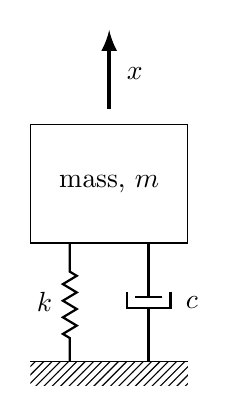
\begin{tikzpicture}
\tikzstyle{spring}=[thick,decorate,decoration={zigzag,pre length=0.3cm,post length=0.3cm,segment length=6}]

\tikzstyle{damper}=[thick,decoration={markings,  
  mark connection node=dmp,
  mark=at position 0.5 with 
  {
    \node (dmp) [thick,inner sep=0pt,transform shape,rotate=-90,minimum width=15pt,minimum height=3pt,draw=none] {};
    \draw [thick] ($(dmp.north east)+(2pt,0)$) -- (dmp.south east) -- (dmp.south west) -- ($(dmp.north west)+(2pt,0)$);
    \draw [thick] ($(dmp.north)+(0,-5pt)$) -- ($(dmp.north)+(0,5pt)$);
  }
}, decorate]

\tikzstyle{ground}=[fill,pattern=north east lines,draw=none,minimum width=2cm,minimum height=0.3cm]


\node [right] at (0.1, 1.4) {$x$};
\node (M) [draw, minimum width=2cm, minimum height=1.5cm] {mass, $m$};

\draw [-latex,ultra thick] (M.north) ++(0,0.2cm) -- +(0,1cm);
%\draw [help lines] (0,0) grid (2,3);

\node (ground1) at (M.south) [ground,yshift=-1.5cm, anchor=north] {};
\draw (ground1.north west) -- (ground1.north east);

\draw [spring] (ground1.north) ++(-0.5, 0) -- (-0.5, -0.75);
\node [left] at (-0.6, -1.5) {$k$};
\draw [damper] (ground1.north) ++(0.5, 0) -- (0.5, -0.75);
\node [right] at (0.85, -1.5) {$c$};


\end{tikzpicture}
\end{figure}

\subsection*{Equation of Motion:}
Simple spring - mass - damper equation of  motion:
\begin{equation*}
	m*\ddot{x} + c*\dot{x} +k*x = 0	
\end{equation*}

where:
\begin{align*}
	x &= \text{displacement - } m\\
	m &= \text{mass - } kg\\
	c &= \text{damping factor - } \frac{N}{m/s}\\
	k &= \text{spring stiffness - } \frac{N}{m}
\end{align*}

Reformulated for only single order equations for use with the RK4 solver:

\begin{align*}
	x &= x_1\\
	\dot{x_1} &= x_2\\
	\dot{x_2} &= -\frac{c}{m}*x_2 -\frac{k}{m} * x_1
\end{align*}
Initial Conditions:
\begin{align*}
	x_1(t_0) &= x_0\\
	x_2(t_0) &= 0
\end{align*}

State Vector:
\begin{equation*}
	State = \begin{bmatrix}
	x_1 \\
	x_2
	\end{bmatrix}
\end{equation*}

\subsection *{Solution Process}
\begin{enumerate}
	\item Define State Equations
	\begin{enumerate}
		\item Initialize array containing equations
	\end{enumerate}
	\item Define initial conditions
	\begin{enumerate}
		\item This is the initial state vector for the system
	\end{enumerate}
	\item Define solution time vector
	\item Solution loop: While $(t <= t_{end})$
	\begin{enumerate}
		\item Solve for new state vector using RK4
		\item Store data
	\end{enumerate}
	
\end{enumerate}

\subsection*{Exact Solution:}
Three different exact solutions are possible for this system based on the system parameters.

\subsubsection*{Underdamped Solution: $\zeta < 1$}
\begin{equation*}
	x(t) = A e^{-\zeta \omega_n t} sin(\omega_dt + \phi)			
\end{equation*}
where:
\begin{align*}
	\omega_n &= \sqrt{\frac{k}{m}} \\
	\zeta &= \frac{c}{2\omega_nm}\\
	\omega_d &= \omega_n \sqrt{1- \zeta^2}	\\
	A &= \frac{\sqrt{(x_0\omega_d)^2 + (v_0 + x_0\zeta\omega_n)^2}}{\omega_d}\\
	\phi &= arctan\frac{x_0\omega_d}{v_0+x_0\zeta\omega_n}
\end{align*}

\subsubsection*{Critically Damped Solution: $\zeta = 1$}		
\begin{equation*}
	x(t) = c_1 e^{-\zeta \omega_n t} + c_2te^{-\zeta \omega_n t}
\end{equation*}
where:
\begin{align*}
	c_1 &= x_0\\
	c_2 &= v_0 + x_0\zeta\omega_n
\end{align*}

\subsubsection*{Overdamped Solution $\zeta > 1$}
\begin{equation*}
	x(t) = e^{-\zeta \omega_n t} \big(c_1e^{\omega_n\sqrt{\zeta^2 -1}t} + c_2e^{-\omega_n\sqrt{\zeta^2-1}t}\big)
\end{equation*}

where:
\begin{align*}
	c_1 = \frac{x_0\omega_n(\sqrt{\zeta^2-1}+\zeta)+ v_0}{2\omega_n\sqrt{\zeta^2-1}}\\
	c_2 = \frac{x_0\omega_n(\sqrt{\zeta^2-1}-\zeta)- v_0}{2\omega_n\sqrt{\zeta^2-1}}\\
\end{align*}


\subsection*{Simulation results:}
Using $m = 1 kg$ and $k = 1000 \frac{N}{m}$ the natural frequency of the system is $\approx5$ $Hz$. Three different values of $c$ are chosen to exercise each results case. 


\includegraphics[scale=0.9]{Under_Damped_Pos}
\includegraphics[scale=0.9]{Under_Damped_Vel}
\includegraphics[scale=0.9]{Critically_Damped_Pos}
\includegraphics[scale=0.9]{Critically_Damped_Vel}
\includegraphics[scale=0.9]{Over_Damped_Pos}
\includegraphics[scale=0.9]{Over_Damped_Vel}

\newpage
\section*{Spring Mass Damper - Forced Input}
This section covers the solution of the forced problem.  The input force is a swept sine signal.

\subsection *{System Diagram:}
\begin{figure}[!h]
\centering

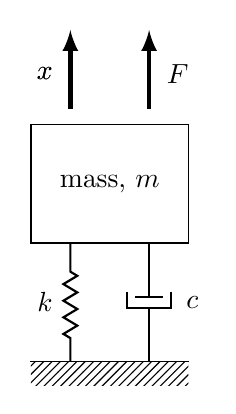
\begin{tikzpicture}
\tikzstyle{spring}=[thick,decorate,decoration={zigzag,pre length=0.3cm,post length=0.3cm,segment length=6}]

\tikzstyle{damper}=[thick,decoration={markings,  
  mark connection node=dmp,
  mark=at position 0.5 with 
  {
    \node (dmp) [thick,inner sep=0pt,transform shape,rotate=-90,minimum width=15pt,minimum height=3pt,draw=none] {};
    \draw [thick] ($(dmp.north east)+(2pt,0)$) -- (dmp.south east) -- (dmp.south west) -- ($(dmp.north west)+(2pt,0)$);
    \draw [thick] ($(dmp.north)+(0,-5pt)$) -- ($(dmp.north)+(0,5pt)$);
  }
}, decorate]

\tikzstyle{ground}=[fill,pattern=north east lines,draw=none,minimum width=2cm,minimum height=0.3cm]



\node (M) [draw, minimum width=2cm, minimum height=1.5cm] {mass, $m$};

\node [left] at (-0.6, 1.4) {$x$};
\draw [-latex,ultra thick] (M.north) ++(-0.5,0.2cm) -- +(0,1cm);
\node [left] at (-0.6, 1.4) {$x$};
\draw [-latex,ultra thick] (M.north) ++(0.5,0.2cm) -- +(0,1cm);
\node [right] at (0.6, 1.4) {$F$};
%\draw [help lines] (0,0) grid (2,3);

\node (ground1) at (M.south) [ground,yshift=-1.5cm, anchor=north] {};
\draw (ground1.north west) -- (ground1.north east);

\draw [spring] (ground1.north) ++(-0.5, 0) -- (-0.5, -0.75);
\node [left] at (-0.6, -1.5) {$k$};
\draw [damper] (ground1.north) ++(0.5, 0) -- (0.5, -0.75);
\node [right] at (0.85, -1.5) {$c$};

\end{tikzpicture}
\end{figure}

\subsection *{Equations of Motion:}
Forced spring - mass - damper equation of  motion:
\begin{equation*}
	m*\ddot{x} + c*\dot{x} +k*x = F	
\end{equation*}
State equation form:
\begin{align*}
	x &= x_1\\
	\dot{x_1} &= x_2\\
	\dot{x_2} &= -\frac{c}{m}*x_2 -\frac{k}{m} * x_1 + \frac{F}{m}
\end{align*}
Linear swept sine wave algorithm (reference: http://www.vibrationdata.com/tutorials/sweep.pdf)
\begin{equation*}
	F(t) = amp * sin(\frac{\pi*f_2*t^2}{t_2})
\end{equation*}

This assumes the starting time and frequency are zero and:
\begin{align*}
	f_2 &= \text{End Frequency - } Hz\\
	t_2 &= \text{End Time - } s\\
	t &= \text{Current Time - } s\\
	amp &= \text{Amplitude - } N
\end{align*}

\subsection *{Solution Process}
\begin{enumerate}
	\item Define State Equations
	\begin{enumerate}
		\item Initialize array containing equations
	\end{enumerate}
	\item Define initial conditions
	\begin{enumerate}
		\item Initial state vector for the system
		\item Initial force on the system
	\end{enumerate}
	\item Define solution time vector
	\item Solution loop: While $(t <= t_{end})$
	\begin{enumerate}
		\item Calculate Force
		\item Store data		
		\item Solve for new state vector using RK4		
	\end{enumerate}
	
\end{enumerate}

\subsection *{Simulation Results}
The results shown below are based on input parameters specifically chosen to set the natural frequency of the system to $\approx5$ $Hz$.  The frequency rate for the sine sweep will be set such that this frequency will be hit at $\approx 15$ $s$ of a $30$ $s$ sweep.

\begin{align*}
	m &= 1 \text{ } kg\\
	c &= 1 \text{ } \frac{N}{m/s}\\
	k &= 1000 \text{ } \frac{N}{m}\\
	t_2 &= 30\text{ }Hz\\
	f_2 &= 10\text{ }s
\end{align*}




\end{document}